%File: formatting-instruction.tex
\documentclass[letterpaper]{article}
\usepackage{aaai}
\usepackage{times}
\usepackage{helvet}
\usepackage{graphicx} 
\usepackage{courier}
\usepackage{listings}
\graphicspath{ {./} }
\frenchspacing
\setlength{\pdfpagewidth}{8.5in}
\setlength{\pdfpageheight}{11in}
\pdfinfo{
/Title (Insert Your Title Here)
/Author (Put All Your Authors Here, Separated by Commas)}
\setcounter{secnumdepth}{0}  
 \begin{document}
% The file aaai.sty is the style file for AAAI Press 
% proceedings, working notes, and technical reports.
%
\title{Tic-Tac-Toe with MiniMax Algorithm}
\author{ Thomas McDonald\\
University of Colorado – Colorado Springs\\
tmcdonal@uccs.edu\\
}
\maketitle
\begin{abstract}
\begin{quote}
This paper entails the challenges of making an artificial intellegent program face off against humans in a game of Tic Tac Toe and my implementation to make a program do so.  
\end{quote}
\end{abstract}

\section{Introduction}
Tic Tac Toe has been a game played by a majority of people throughout many generations Some people think this game was  invented at Ancient Egypt, and then Roman Empire called this game “Terni Lapili”. The grid drawing for the game had been found chalked all over the ancient city’s ruins ~\cite{unknown}. Tic Tac Toe contains a 3x3 grid where the players alternate between picking a sqaure in the grid with a unuiqe symbol; usually one individual has an X to place on their turn while the other places an O on there selected spot. The goal of the game is to get 3 symbols in a row whether it be horizontally, diagonaly, or vertically. As soon as a player gets three in a row, the game is over with the winner defined as the player that was able to get three symbols in a row. There is a possibility that no one wins after there are no available choices for a player to pick resulting the game to be a draw. Tic Tac Toe was one of the starting points for primitive AI. A computer must make rational decisions when playing the game in order to beat the opponent. Developed as one of the very first video games ~\cite {wikes}, computer scientists were able to acomplish implementing an AI that can interactively challenge humans to the game of Tic Tac Toe. With the advancement of computing power, new and evolving methods of making an artificial opponent has come forth. To demonstrate some of the progress human beings have made towards making a worthy opponent, I will be implementing an AI that uses the MiniMax algorithm that decides the best possible moves to challenge an opponent in both the traditional game of tic-tac-toe and a version where its a 3x3x3 game of tic-tac-toe.

\section{Background}
Since the dawn of video games, AI has been needed to challenge the player and keep them hooked to the game. As a matter of fact, Tic Tac Toe was one of the first video games created on the ESDAC computer with an AI capaable of defeating oponents ~\cite{beck}. The evolution of AI techniques continues to advance. Alot of the newer game theory algorithms and artifial intelligence algorithms devised can still be applied to Tic Tac Toe just like they can be applied to multiple games like chess or go. This makes the selection of picking a method for a Tic Tac Toe AI difficult because the wide varieties of implementation others have carried out. Computer scientists will always continue improving the teqniques used to solve the problem, which shows true for the way of improving the AI behind Tic Tac Toe video games.

\section{Challenges}
The game of Tic Tac Toe is easy at a glimpse, but making a computer go through the same thought processes that humans go through before a decision gets complex quickly. Cosidering there are 9 spots that can be filled with an X, O, or Blank spot, there are 19,683 possible states ~\cite {garg_2017}. This of course, is not including the restrictions of the number of symbols that can be placed in an turn by turn scenario. An AI must be able navigate through all possible states and simultatiously play in a way that gets it to a subset where the state results in a win for the AI. The entity most know all possible states as its playing or must be able to dynamically choose what to do based on the current state of the board. With the 3x3x3 board, the game gets even more complex with $3^(9*3) = 7,625,597,484,987$ possible configurations. This huge state space becomes a problem since there is no way a playable AI can consider 7,625,597,484,987 possible configurations in a playable game.

\section{Method of Implementation for traditional Tic-Tac-Toe}
\subsection{MiniMax Algorithm}
The minimax algorithm has been in the game industry for quite some time and can be applied to other strategic games like chess or go ~\cite {inproceedings}. The minimax algorithm finds optimal decisions to take by maximizing its chances of winning by minimizing the oponents chances of winning. In other words, it looks ahead and sees what possible moves its opponent can make, and makes a decision that minimizes the damage the oppenent can do. Roopali Garg and Deva Prasad Nayak prove the application of minimax being useful for tic tac toe by fully implementing it and demonstating the computer either ending up in a draw state or beating the human opponent. Since the game of Tic Tac Toe isn’t as complex as something like chess or go,  The minimax algorithm is the way to go. With the memory capabilities we have today, the second the opponent makes a decision, our program will be several steps ahead of them. Also, since we only have a couple months to complete this model and a lot of effort has to also go into making a playable game, it’s only appropriate to consider this method since it is doable in such a short time frame opposed to doing something complex like a genetic neural network with double transfer functions which would take the construction of a nueral net alongside training it. Lets not forget that the minimax algorithm takes a whole lot less of the resources compared to the other methods of implementation.   

\subsection{Implementing MiniMax with Tic Tac Toe}
I wrote my playable implementation of MiniMax with python. Python's portability makes the showcase of my code as easy as possible to demonstrate on different environments without the hassle of making sure the environment has the correct requirements beforehand. The board I'm using for this program is made up of 3 seperate lists within a list. Each list within the list represents the 1st,2nd, and 3rd row of a Tic Tac Toe game board. The program consists of first initializing the board with the computer taking the first move. It's proven that the corners are the highest advantaged first move, so to make this AI unbeatable, I initialized the computers first move as the top left corner ~\cite {wolframdemonstrationsproject_2007}. From there, the opponent playing the program is to make a move. I have the moves you can make as a pair of co-ordinates where 0,0 is taken by the computer, 1,1 is the center of the board 2,2 is the bottom right corner, and so on. The players move looks like so:
\begin{lstlisting}
['X', '-', '-']
['-', '-', '-']
['-', '-', '-']
Enter your move (x, y)
\end{lstlisting}
After the player makes a move, the computer must now pick the best possible next move. To do so, the computer calls the miniMax funtion I have defined. The miniMax funtion starts by checking all possible moves for the current player, which in this case, is the AI. To find each and every possible move the player can make, I parse through the board for any '-' symbols and return a list of co-ordinates representing the moves the player can make.
\begin{lstlisting}
def possibleMoves(board):
    moves = []
    index = 0
    for i in board:
        for j in range(len(i)):
            if i[j] == '-':
                moves.append([j,index])
        index = index +1
    return moves                
\end{lstlisting}
 For each possible move, the computer recursively calls the miniMax funtion again and changes the current player to the opponent so the opponent's moves can be calculated. The Function will keep calling itself until the board passed in is in a winning state for either players, or until there is no possible moves left. Once we reach the final states of the recursive calls, the function returns a score of 1 if the computer wins in this state, a -1 if the opponent wins in this state, and a 0 for no winner.Checking the score of the board passed in was fairly straight forward as shown below.
\begin{lstlisting}
def checkScore(board):
    columns = [[],[],[]]
    diagonals = [[],[]]
    for i in board:
        columns[0].append(i[0])
        columns[1].append(i[1])
        columns[2].append(i[2]) 
    diagonals[0].append(board[0][0])
    diagonals[0].append(board[1][1])
    diagonals[0].append(board[2][2])
    diagonals[1].append(board[0][2])
    diagonals[1].append(board[1][1])
    diagonals[1].append(board[2][0])
    for i in board:
        if i[0] == 'X' and i[1] == 'X'
	\ and i[2] == 'X':
            return 1
        elif i[0] == 'O' and i[1] == 'O'
	\ and i[2] == 'O':
            return -1

    for i in columns:
        if i[0] == 'X' and i[1] == 'X'
	\ and i[2] == 'X':
            return 1
        elif i[0] == 'O' and i[1] == 'O' 
	\ and i[2] == 'O':
            return -1

    for i in diagonals:
        if i[0] == 'X' and i[1] == 'X'
	\ and i[2] == 'X':
            return 1
        elif i[0] == 'O' and i[1] == 'O'
	\ and i[2] == 'O':
            return -1
    return 0
\end{lstlisting}
Each possible move now has a score associated with the state of the board passed in. For the computers prespective, I make the computer only pick states that land the board in either winning or a draw state. For the opponent, the opponent tries to only pick moves that garuantee it's win. The final result returns a list of co-ordinates for the computer to make in its next move. The AI makes the move and the game is back into the player's hands. After each move the player makes, the computer again uses miniMax with the current state of the board to again decide the best course of action for itself. Once the game see's itself in a win state, the player with the consecutive symbols is displayed to the user. 

\subsection {Final Thoughts}
MiniMax proved to be a useful algorithm to apply to traditional Tic Tac Toe. In some cases however, I have seen the AI make some apparently irrational decisions. One pitfall of the MiniMax algorithm is that the algorithm assumes that the opponent will play optimally. When the opponent makes irrational decisions, the computer makes the best move of what it can make out of the situation, which might not be something a human would do. Take this sequence of moves for example:
\begin{lstlisting}
['X', '-', '-']
['-', '-', '-']
['-', '-', '-']
Enter your move (x, y)
1,0
['X', 'O', '-']
['-', '-', '-']
['X', '-', '-']
Enter your move (x, y)
2,0
['X', 'O', 'O']
['-', '-', '-']
['X', '-', 'X']  
\end{lstlisting}
Here on the second move I made irrational move of placing my symbol on the top right instead of blocking the potential win. Any human with some sense would complete the three 'X's in a row but the MiniMax algorithm makes a defensive move instead. Here you can see how the computer was expecting the opponent to play optimally and had a unusual move as a result of the opponent not playing optimally. Although the AI makes some of these apparently quirky decisions, the outcome always has the AI as the winner since each and every move the computer makes is playing both defensivley and offensively. In the example I gave above, yes the computer did not grab the immediate win, but, instead it made the win it can have in the next moves a garauntee. In the end, I haven't been able to beat my own implementation which is what I was hoping for. The robustness of MiniMax has proven it's worth. My implementation has a corresoponding move almost immediately and has yet to be beaten. Hopefully, the MiniMax algorithm can follow suit once we implement the 3x3x3 game of Tic Tac Toe.

\section{Method of Implementation for 3x3x3 Tic-Tac-Toe}
\subsection{MiniMax Algorithm with Alpha Beta Pruning}
The minimax algorithm was very robust in my initial implementation, however, when trying to implement the same algorithm on a 3x3x3 board, the algorithm would hang on trying to compute all possible moves the computer and a player playing optimally could make. This is usually the case when using minimax, minimax can be applied to database systems, expert systems, robot control systems, and theorem-provers but usually has to be adapted to handle the large state space that accompanies the problem at hand ~\cite{boro}. When trying to reduce the number of nodes to traverse in a tree, a common solution is to prune your tree while traversing. As anyone who knows MiniMax would suggest, the solution to this problem would be to use Alpha Beta pruning. As S. H. Fuller, J. G. Gaschnig and J. J. Gillogly state, "Alpha-beta is faster than mini-max because it does not explore some branches of the tree that will not affect the backed-up value" ~\cite{fullegaschnigillogly1973}. Alpha Beta pruning also utilizes the depth of the recursive function, allowing you to limit the amount of computation you've deemed neccessary for your AI making it perfect to adapt and test the level of diffuclty the AI can have. 

\subsection{Implementing MiniMax with Alpha Beta Pruning for 3x3x3 Tic Tac Toe}
As before, I wrote my playable implementation of MiniMax using the programming language python. I chose python because the simplicity of the syntax and the robustness of python's variable typing. Python's portability and readability makes the showcase of my code as easy as possible to demonstrate on different environments without the hassle of making sure the environment has the correct requirements beforehand. Before I could implement anything, I had to set up how the game would be playable. To begin, I had to create a board. My representation of the board is an array of 3 tic-tac-toe boards where each index represents a layer in the tic-tac-toe cube. For example, when the game starts you are shown the state of the board with the computer making the first move.
\begin{lstlisting}
 Layer 0 in board:
['-', '-', '-']
['-', '-', '-']
['-', '-', '-']
Layer 1 in board:
['-', '-', '-']
['-', 'X', '-']
['-', '-', '-']
Layer 2 in board:
['-', '-', '-']
['-', '-', '-']
['-', '-', '-']
Enter your move i.e: x, y, z
\end{lstlisting}
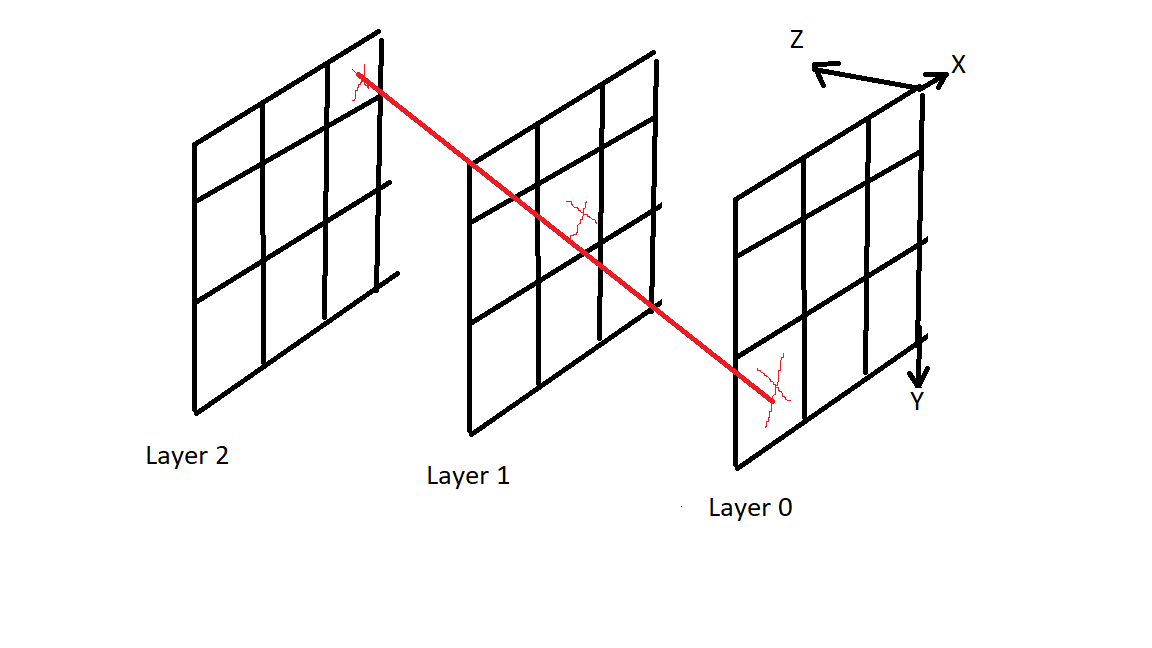
\includegraphics [scale=0.2] {board}

The X,Y, and Z axis are shown in the image above to better help you visualize the board and the respective axis. I hardcoded the center move as the computers first move to ensure the computer always wins. It is proven that the center as a first move has an unfair advantage to win compared to all other possible initial moves ~\cite{felstiner2019}. An important part of this utilizing MiniMax is to know all possible moves given a board state. I do this with my checkMoves function that works as followed:
\begin{lstlisting}
def possibleMoves(board):
    moves = []
    y = 0
    z = 0
    for layer in board:
        y=0
        for i in layer:
            for x in range(len(i)):
                if i[x] == '-':
                    moves.append([x,y,z])
            y = y +1
        z=z+1
    return moves 
\end{lstlisting}

The next step to building the game was detecting if the board at hand is in a winning state. Win states include any win state for each layer, treating the layer as a traditional game of tic-tac-toe, and win states across the Z axis. To detect if the board is in a win state, I use the checkWin() function that I created. The last part of setting up the game was creating a checkScore() function that returns the 3 if the computer is in a win state, or a -3 if the opponent is in a win state. If neither player is in a win state, the function returns a 0. After all the inital setup, the MiniMax algorithm with Alpha Beta Pruning was ready to implement. Here's a snapshot of my MiniMax algorithm. 
\begin{lstlisting}
def miniMax(board,maximizer, depth):
    if depth == 3:
        return [checkScore(board),[]]

    if maximizer:
        best = -10000000
        moves = possibleMoves(board)
        if moves:
            bestMove = []
            for i in moves:
                temp = copy.deepcopy\
				(board)
                temp[i[2]][i[1]][i[0]] =\
 				'X'
                value = [-10000000, []]
                if checkWin(temp):
                    best = 7-depth
                    bestMove = i
                else:
                    value = miniMax\
		(temp, False, depth+1)
                if value[0] > best:
                    best = value[0]
                    bestMove = i
            return [best, bestMove]
    else:
        best = 10000000
        moves = possibleMoves\
		(board)
        if moves:
            bestMove = []
            for i in moves:
                temp = copy.\
			deepcopy(board)
                temp[i[2]][i[1]][i[0]]\
 				= 'O'
                value = [10000000,\
 				[]]
                if checkWin(temp)\
 				== True:
                    best = depth-7
                    bestMove = i
                else:
                    value = \
	miniMax(temp, True, depth+1)
                if value[0] < best:
                    best = value[0]
                    bestMove = i
            return [best, bestMove]
\end{lstlisting}
The algorithm is looking 3 moves ahead, alternating between its best possible moves and the oponents best possible moves. To make the tree prune, I use the recursive depth to penalize moves that are further ahead. For example, with the traditional minimax algorithm the computer could have a move that ensures a win thats 10 moves ahead, or a win thats only one move away and the computer could pick the move that is 10 moves ahead instead of grabbing an immediate win. To prioritize the closer moves, I ensured the score was higher if it was less deep than the other possible moves much like Ronald L. Rivest's description on Penalty-based iterative search methods ~\cite{rivest1987}. As soon as the algorithm sees a win state, I return the score and prune the other possibilities, since a win state is the most prioritized possibility. Doing this fixed my problem from the traditional game of tic-tac-toe where if the player does not play optimally, the computer would pick seemingly random moves instead of winning. 
\subsection {Demonstration}
Here's a game played against the AI:
\begin{lstlisting}
 Layer 0 in board:
['-', '-', '-']
['-', '-', '-']
['-', '-', '-']
Layer 1 in board:
['-', '-', '-']
['-', 'X', '-']
['-', '-', '-']
Layer 2 in board:
['-', '-', '-']
['-', '-', '-']
['-', '-', '-']
Enter your move i.e: x, y, z 
1,1,2
Layer 0 in board:
['X', '-', '-']
['-', '-', '-']
['-', '-', '-']
Layer 1 in board:
['-', '-', '-']
['-', 'X', '-']
['-', '-', '-']
Layer 2 in board:
['-', '-', '-']
['-', 'O', '-']
['-', '-', '-']
Enter your move i.e: x, y, z 
2,2,2
Layer 0 in board:
['X', '-', '-']
['-', '-', '-']
['-', '-', '-']
Layer 1 in board:
['-', '-', '-']
['-', 'X', '-']
['-', '-', '-']
Layer 2 in board:
['X', '-', '-']
['-', 'O', '-']
['-', '-', 'O']
Enter your move i.e: x, y, z
2,2,0
Final Board:
Layer 0 in board:
['X', '-', '-']
['-', '-', '-']
['-', '-', 'O']
Layer 1 in board:
['X', '-', '-']
['-', 'X', '-']
['-', '-', '-']
Layer 2 in board:
['X', '-', '-']
['-', 'O', '-']
['-', '-', 'O']
youre a loser
\end{lstlisting}

\subsection {Final Thoughts}
The game AI performs very well and to the best of my knowledge is unbeatable. I have yet to win a game against it. Limiting the depth of my tree alleviated alot of unecessary computation, making the AIs response seemingly instant. If I were to continue this project, I'd add a difficulty parameter that sets the depth of the recursion so the player can play with different versions of the AI making it harder or easier to play against.


\bibliographystyle {unsrt}
\bibliography{bibl}

\end{document}